
\noindent\begin{minipage}{\textwidth}
    \begin{table}[H]
        \centering
        \caption{Hiperparâmetros e Resultados do Melhor Modelo - densenet\_v1\_AB\_opt\_aug}
        \vspace{0.2cm}
        \resizebox{\textwidth}{!}{%
            \begin{tabular}{ll | lrrr}
                \hline
                \multicolumn{2}{c|}{\textbf{Hiperparâmetros}} & \multicolumn{4}{c}{\textbf{Métricas por Classe}} \\ \hline
                \textbf{Parâmetro} & \textbf{Valor} & \textbf{Classe} & \textbf{Precisão} & \textbf{Recall} & \textbf{F1-Score} \\ \hline
    Agendador (Patience) & 7 & 31.2 & 0.5206 & 0.8938 & 0.6580 \\ 
Agendador de LR & ReduceLROnPlateau & 31.3 & 0.7843 & 0.3960 & 0.5263 \\ 
Architecture & densenet121 & 31.4 & 0.5403 & 0.6381 & 0.5852 \\ 
Augmentation (Método) & None & 32.3 & 0.6609 & 0.7857 & 0.7179 \\ 
Batch Size & 32 & 32.4 & 0.9565 & 0.3793 & 0.5432 \\ 
Decaimento de Peso (WD) & 0.0009 & 33.3 & 0.8559 & 0.5233 & 0.6495 \\ 
Dropout & 0.2026 & 41.4 & 0.6471 & 0.5000 & 0.5641 \\ 
Função de Perda & CrossEntropyLoss & 41.5 & 0.6809 & 0.8205 & 0.7442 \\ 
Hidden Units & 512 & 42.4 & 0.7959 & 0.5735 & 0.6667 \\ 
Label Smoothing & 0.1000 & 44.4 & 0.8261 & 0.6552 & 0.7308 \\ 
\cline{3-6} 
Otimizador & AdamW & \textbf{Média (Macro)} & 0.6829 & 0.6429 & 0.6497 \\ 
Taxa de Aprendizado (LR) & 1.51e-04 & \textbf{MCC} & \multicolumn{3}{c}{0.6031} \\ 
Unfreeze Layers & 2 &  & & &  \\ 
            \hline
            \end{tabular}%
        }
    \end{table}

    \begin{figure}[H]
        \centering
        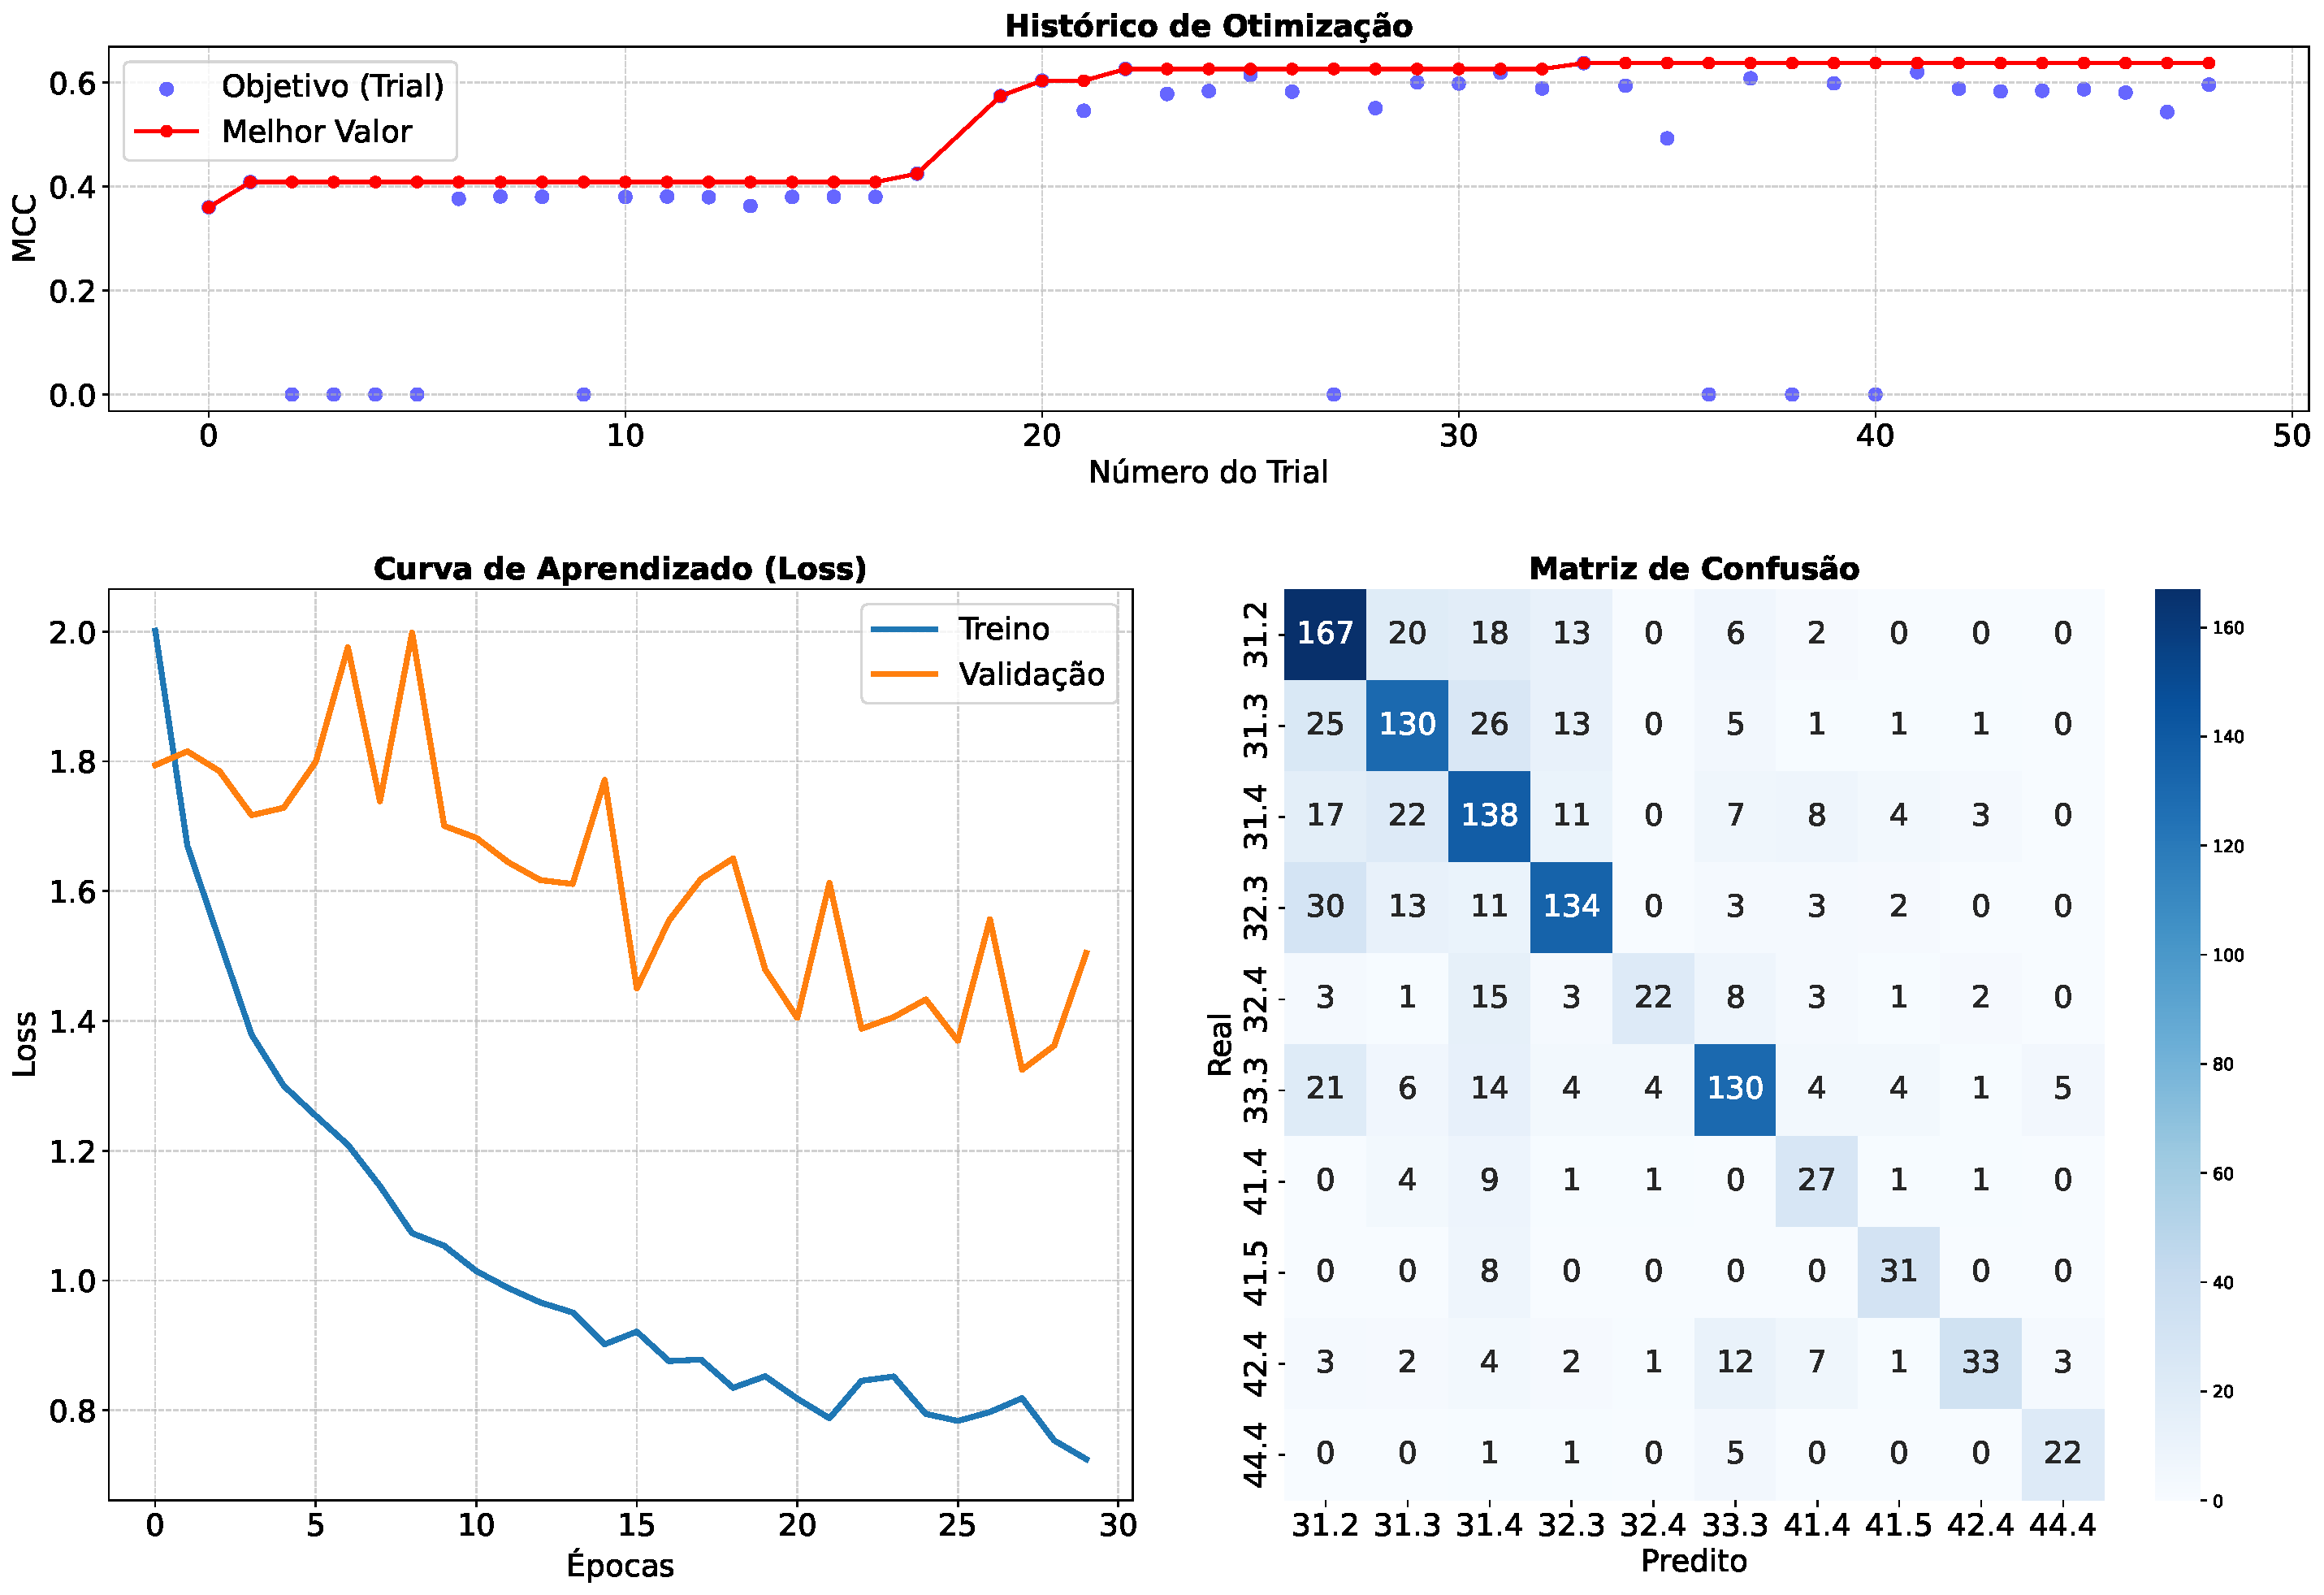
\includegraphics[width=0.9\textwidth]{tex/appendix/experiments/densenet_v1_AB_opt_aug/dashboard_consolidado.pdf}
        \caption{Histórico de Otimização, Curvas de Aprendizado e Matriz de Confusão - densenet\_v1\_AB\_opt\_aug}
    \end{figure}
\end{minipage}

\clearpage
\pdfpagewidth=297mm \pdfpageheight=210mm
\newgeometry{left=1.5cm, right=1.5cm, top=2.5cm, bottom=2cm} 
\begin{figure}[H]
    \centering
    \makebox[\textwidth][l]{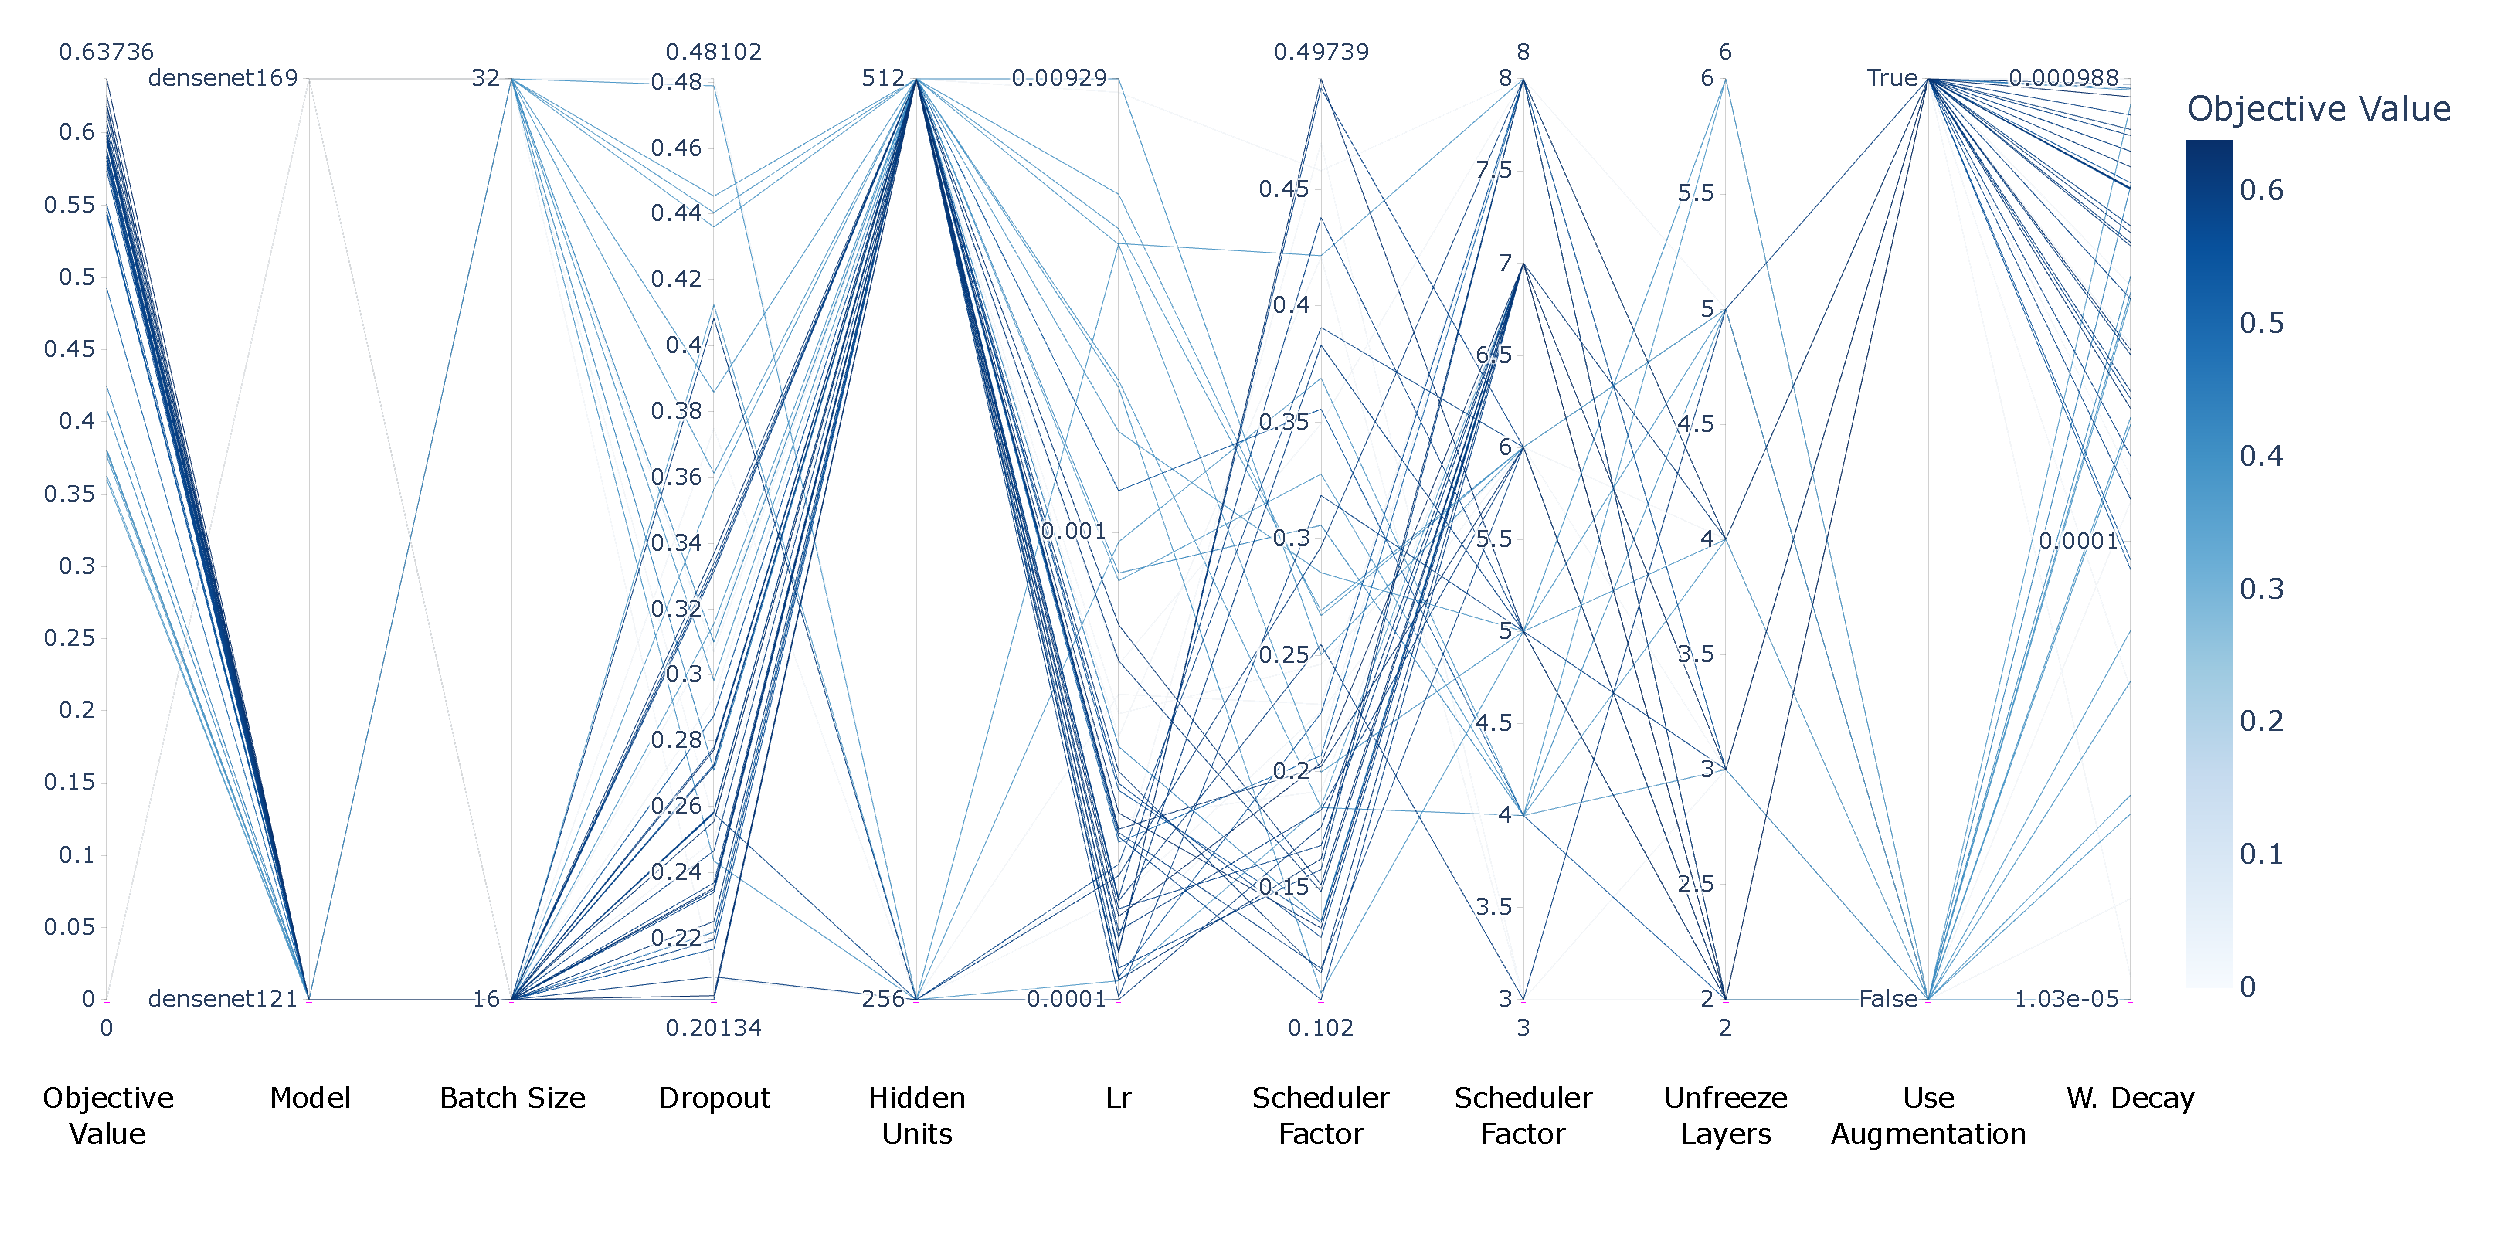
\includegraphics[width=1.7\textwidth]{tex/appendix/experiments/densenet_v1_AB_opt_aug/optuna_parallel.pdf}}
    \caption{Coordenadas Paralelas dos principais hiperparâmetros para densenet\_v1\_AB\_opt\_aug}
\end{figure}
\clearpage
\pdfpagewidth=210mm \pdfpageheight=297mm
\restoregeometry
\newpage
